\documentclass[a4paper]{article}

\usepackage{inputenc}
\usepackage[british,UKenglish]{babel}
\usepackage{amsmath}
%\usepackage{titlesec}
\usepackage{color}
\usepackage{graphicx}
\usepackage{fancyref}
\usepackage{hyperref}
\usepackage{float}
\usepackage{scrextend}
\usepackage{setspace}
\usepackage{xargs}
\usepackage{multicol}
\usepackage{nameref}

\usepackage{sectsty}
\usepackage{multicol}
\usepackage{multirow}
\usepackage[procnames]{listings}
\usepackage{appendix}

\newcommand\tab[1][1cm]{\hspace*{#1}}
\hypersetup{colorlinks=true, linkcolor=black}
\interfootnotelinepenalty=10000

\newcommand{\cleancode}[1]{\begin{addmargin}[3em]{3em}\texttt{\textcolor{cleanOrange}{#1}}\end{addmargin}}
\newcommand{\cleanstyle}[1]{\text{\textcolor{cleanOrange}{\texttt{#1}}}}


\usepackage[colorinlistoftodos,prependcaption,textsize=footnotesize]{todonotes}
\newcommandx{\commred}[2][1=]{\textcolor{Red}
{\todo[linecolor=red,backgroundcolor=red!25,bordercolor=red,#1]{#2}}}
\newcommandx{\commblue}[2][1=]{\textcolor{Blue}
{\todo[linecolor=blue,backgroundcolor=blue!25,bordercolor=blue,#1]{#2}}}
\newcommandx{\commgreen}[2][1=]{\textcolor{OliveGreen}{\todo[linecolor=OliveGreen,backgroundcolor=OliveGreen!25,bordercolor=OliveGreen,#1]{#2}}}
\newcommandx{\commpurp}[2][1=]{\textcolor{Plum}{\todo[linecolor=Plum,backgroundcolor=Plum!25,bordercolor=Plum,#1]{#2}}}

\def\code#1{{\tt #1}}

\def\note#1{\noindent{\bf [Note: #1]}}

\makeatletter
%% The "\@seccntformat" command is an auxiliary command
%% (see pp. 26f. of 'The LaTeX Companion,' 2nd. ed.)
\def\@seccntformat#1{\@ifundefined{#1@cntformat}%
   {\csname the#1\endcsname\quad}  % default
   {\csname #1@cntformat\endcsname}% enable individual control
}
\let\oldappendix\appendix %% save current definition of \appendix
\renewcommand\appendix{%
    \oldappendix
    \newcommand{\section@cntformat}{\appendixname~\thesection\quad}
}
\makeatother


% "define" Scala
\usepackage[T1]{fontenc}  
\usepackage[scaled=0.82]{beramono}  
\usepackage{microtype} 

\sbox0{\small\ttfamily A}
\edef\mybasewidth{\the\wd0 }

\lstdefinelanguage{scala}{
  morekeywords={abstract,case,catch,class,def,%
    do,else,extends,false,final,finally,%
    for,if,implicit,import,match,mixin,%
    new,null,object,override,package,%
    private,protected,requires,return,sealed,%
    super,this,throw,trait,true,try,%
    type,val,var,while,with,yield},
  sensitive=true,
  morecomment=[l]{//},
  morecomment=[n]{/*}{*/},
  morestring=[b]",
  morestring=[b]',
  morestring=[b]"""
}

\usepackage{color}
\definecolor{dkgreen}{rgb}{0,0.6,0}
\definecolor{gray}{rgb}{0.5,0.5,0.5}
\definecolor{mauve}{rgb}{0.58,0,0.82}

% Default settings for code listings
\lstset{frame=tb,
  language=scala,
  aboveskip=3mm,
  belowskip=3mm,
  showstringspaces=false,
  columns=fixed, % basewidth=\mybasewidth,
  basicstyle={\small\ttfamily},
  numbers=none,
  numberstyle=\footnotesize\color{gray},
  % identifierstyle=\color{red},
  keywordstyle=\color{blue},
  commentstyle=\color{dkgreen},
  stringstyle=\color{mauve},
  frame=single,
  breaklines=true,
  breakatwhitespace=true,
  procnamekeys={def, val, var, class, trait, object, extends},
  procnamestyle=\ttfamily\color{red},
  tabsize=2
}

\lstnewenvironment{scala}[1][]
{\lstset{language=scala,#1}}
{}
\lstnewenvironment{cpp}[1][]
{\lstset{language=C++,#1}}
{}
\lstnewenvironment{bash}[1][]
{\lstset{language=bash,#1}}
{}
\lstnewenvironment{verilog}[1][]
{\lstset{language=verilog,#1}}
{}



\graphicspath{ {images/} }
\usepackage{ctex}
\usepackage{graphicx}
\usepackage{color,framed}%文本框
\usepackage{listings}
\usepackage{caption}
\usepackage{amssymb}
\usepackage{enumerate}
\usepackage{xcolor}
\usepackage{bm} 
\usepackage{lastpage}%获得总页数
\usepackage{fancyhdr}
\usepackage{tabularx}  
\usepackage{geometry}
\usepackage{graphics}
\usepackage{subfigure}
\usepackage{float}
\usepackage{pdfpages}
\usepackage{pgfplots}
\pgfplotsset{width=10cm,compat=1.9}
\usepackage{multirow}
\usepackage{footnote}
\usepackage{booktabs}

%-----------------------伪代码------------------
\usepackage{algorithm}  
\usepackage{algorithmicx}  
\usepackage{algpseudocode}  
\floatname{algorithm}{Algorithm}  
\renewcommand{\algorithmicrequire}{\textbf{Input:}}  
\renewcommand{\algorithmicensure}{\textbf{Output:}} 
\usepackage{lipsum}  
\makeatletter
\newenvironment{breakablealgorithm}
  {% \begin{breakablealgorithm}
  \begin{center}
     \refstepcounter{algorithm}% New algorithm
     \hrule height.8pt depth0pt \kern2pt% \@fs@pre for \@fs@ruled
     \renewcommand{\caption}[2][\relax]{% Make a new \caption
      {\raggedright\textbf{\ALG@name~\thealgorithm} ##2\par}%
      \ifx\relax##1\relax % #1 is \relax
         \addcontentsline{loa}{algorithm}{\protect\numberline{\thealgorithm}##2}%
      \else % #1 is not \relax
         \addcontentsline{loa}{algorithm}{\protect\numberline{\thealgorithm}##1}%
      \fi
      \kern2pt\hrule\kern2pt
     }
  }{% \end{breakablealgorithm}
     \kern2pt\hrule\relax% \@fs@post for \@fs@ruled
  \end{center}
  }
\makeatother
%------------------------代码-------------------
\usepackage{xcolor} 
\usepackage{listings} 
%代码段设置
\lstset{numbers=left,
basicstyle=\tiny,
numberstyle=\tiny,
keywordstyle=\color{blue!70},
commentstyle=\color{red!50!green!50!blue!50},
frame=single, rulesepcolor=\color{red!20!green!20!blue!20}
}


%-------------------------页面边距--------------
\geometry{a4paper,left=2.3cm,right=2.3cm,top=2.7cm,bottom=2.7cm}
%-------------------------页眉页脚--------------
\usepackage{fancyhdr}
\pagestyle{fancy}
\lhead{\kaishu \leftmark}
% \chead{}
\rhead{\kaishu 软件工程实验报告}%加粗\bfseries 
\lfoot{}
\cfoot{\thepage}
\rfoot{}
\renewcommand{\headrulewidth}{0.1pt}  
\renewcommand{\footrulewidth}{0pt}%去掉横线
\newcommand{\HRule}{\rule{\linewidth}{0.5mm}}%标题横线
\newcommand{\HRulegrossa}{\rule{\linewidth}{1.2mm}}
\setlength{\textfloatsep}{10mm}%设置图片的前后间距
%--------------------文档内容--------------------

\begin{document}
\renewcommand{\contentsname}{目\ 录}
\renewcommand{\appendixname}{附录}
\renewcommand{\appendixpagename}{附录}
\renewcommand{\refname}{参考文献} 
\renewcommand{\figurename}{图}
\renewcommand{\tablename}{表}
\renewcommand{\today}{\number\year 年 \number\month 月 \number\day 日}

%-------------------------封面----------------
\begin{titlepage}
    \begin{center}
    
\includegraphics[width=0.8\textwidth]{NKU.png}\\[1cm]
    \vspace{20mm}
		\textbf{\huge\textbf{\kaishu{计算机学院}}}\\[0.5cm]
		\textbf{\huge{\kaishu{软件工程实验报告}}}\\[2.3cm]
		\textbf{\Huge\textbf{\kaishu{结对编程}}}

		\vspace{\fill}
    
    % \textbf{\Large \textbf{并行程序设计期末实验报告}}\\[0.8cm]
    % \HRule \\[0.9cm]
    % \HRule \\[2.0cm]
    \centering
    \textsc{\LARGE \kaishu{姓名\ :\ 平世龙,姚翙载}}\\[0.5cm]
    \textsc{\LARGE \kaishu{年级\ :\ 2020级}}\\[0.5cm]
    \textsc{\LARGE \kaishu{专业\ :\ 计算机科学与技术}}\\[0.5cm]
    
    \vfill
    {\Large \today}
    \end{center}
\end{titlepage}

\renewcommand{\thefigure}{\thesection{}.\arabic{figure}}%图片按章标号
\renewcommand{\abstractname}{\textbf{\large{摘\quad 要}}}
\renewcommand{\figurename}{图}
\renewcommand{\contentsname}{目录}  
\cfoot{\thepage\ of \pageref{LastPage}}%当前页 of 总页数

% 生成目录
\clearpage
\tableofcontents
\newpage

%--------------------------Title--------------------------------
\section{用户手册}
\subsection{引言}
\subsubsection{编写目的}
本用户手册旨在为用户提供使用数独程序的详细说明和指导。该程序旨在帮助用户解决数独难题,提供数独游戏的娱乐和挑战。通过本手册,您将了解程序的功能、界面和使用方法,以便能够充分利用数独程序并提高解决数独问题的效率。无论您是打算使用数独程序解决难题还是寻求数独游戏的乐趣,本手册都将提供您所需的信息和指导。

通过本手册,您将了解以下内容:
\begin{enumerate}
\item 程序的安装和配置要求
\item 软件功能与目标的介绍
\item 软件具体输入输出的格式
\item 程序运行方法与参数说明
\item 源文件的说明
\end{enumerate}
\subsubsection{项目背景}
\begin{enumerate}
\item 项目名称:数独控制台小程序
\item 开发者:本软件工程小组
\item 用户:南开大学师生
\end{enumerate}
\subsection{软件概述}
\subsubsection{目标}
本软件的目标是提供一个简单轻量的数独游戏控制台程序,以满足软件工程课程对程序设计作业的需求。通过该程序,用户可以通过控制台输入参数并运行程序,实现数独游戏的生成、终盘的生成以及游戏的求解等主要功能。为了达到目标,本软件注重以下几个方面:
\begin{enumerate}
\item 简单轻量:本软件设计追求简洁性和轻量化,使得用户可以快速上手并且能够顺利完成所需的数独游戏操作。用户不需要安装复杂的图形界面或其他依赖项,只需在控制台输入相应的命令即可进行游戏操作。
\item 数独功能:软件主要聚焦于数独游戏的核心功能。用户可以通过输入参数来生成新的数独游戏,包括选择游戏的难度级别、指定已知数字的数量等。程序还提供了生成数独终盘的功能,用户可以在生成的游戏基础上进行游戏求解。
\item 用户友好性:尽管本软件是一个控制台程序,但仍致力于提供用户友好的操作体验。通过清晰的命令提示和详细的说明,用户可以轻松理解和使用程序的各项功能。同时,程序会对用户输入进行合理性检查,并给出相应的错误提示,以确保用户能够顺利完成操作。
\item 符合作业需求:本软件旨在满足软件工程课程对程序设计作业的要求,包括输入参数的处理、游戏生成和求解算法的实现等。通过使用本软件,用户能够学习和实践相关的程序设计概念和技术,提高编程能力和理解算法的能力。

\end{enumerate}

\subsubsection{功能}
本软件的功能包括:
\begin{enumerate}
\item 生成数独终盘:用户可以通过软件生成指定数量的数独终盘,并将其输出到文本文件中。这些生成的终盘可作为数独游戏的基础,供用户挑战和解答。
\item 生成数独游戏:软件支持通过挖空法生成数独游戏。用户可以指定挖空的数量范围,从而控制游戏的难度。此外,用户还可以选择生成不同难度级别的游戏,包括简单、中等和困难。对于需要解唯一的游戏,软件也提供了相应的选项。
\item 数独游戏求解:用户可以从文本文件中读取数独游戏,并使用软件进行求解。软件将自动解析数独游戏并找到解,然后将解输出到另一个文本文件中。这个功能可以帮助用户解答难题或验证自己的解答是否正确。
\end{enumerate}
通过这些功能,用户可以充分享受数独游戏的乐趣和挑战。无论是生成终盘、创建自定义难度的游戏,还是使用软件来解答难题,本软件都为用户提供了便捷的操作方式和功能选项。用户可以根据自己的喜好和需求,灵活地使用软件,并享受数独游戏带来的智力训练和娱乐体验。

\subsubsection{运行环境与安装流程}
Win10系统下测试正常运行。本软件不需要复杂的安装流程,只需要保证软件的可执行文件所在位置下,所需的相对输入输出路径均存在即可。
\subsection{数据}
\subsubsection{数据背景}
在本软件下,数据的输入与输出均以txt文件存储。数据完全按照数独游戏的数字进行存储,并且数据的存储适当穿插了空格与空行以增加对用户的可读性。
\subsubsection{输入}
输入文件只包含txt文件,其中:
\begin{enumerate}
\item 每个数独游戏为9行9列的数字+符号+空格组合,其中数字代表游戏中的数字,符号‘\$’代表数独游戏需要填入的空白格。如果是生成的终局或解,则没有符号‘\$’。每个数字与空白格左右均与相邻的数字或空白格以空格隔开,这样组成了一个数独游戏。注意每行最右边以空格结尾。例如:
\begin{lstlisting}
6 8 4 1 9 $ 7 2 $ 
2 5 7 4 $ $ $ $ $ 
$ $ $ 5 7 $ $ 4 8 
3 $ 6 $ $ 8 $ 5 1 
9 $ 5 2 $ 1 $ $ 3 
4 $ $ 9 3 $ $ 6 $ 
$ $ $ 6 $ 7 5 3 $ 
$ $ $ $ 5 4 1 $ $ 
$ $ 2 $ $ $ 8 7 $
\end{lstlisting}
\item 一个文件中有若干个游戏,每个游戏之间以空行分割,文件以空行结束。
\end{enumerate}
\subsubsection{输出}
除了参数'-s'之外,输出文件与输入文件的组织形式相同。
\par
'-s'的参数意义为读取游戏、生成解并输出到文件中,其输出文件也为txt文件,其中输出文件的每个游戏中只包含求解后的所有数字,不包含符号‘\$’。此外,为了处理一个数独游戏有多个解的情况,'-s'输出文件总的组织形式如下:对应读取的文件中的每一个数独游戏,首先输出:'Number of solutions: \$n',其中n为该游戏的解的个数;然后在第二行,依次按照与输入文件格式相同的方法输出所有的解。循环上述步骤直到读取的文件中所有游戏的解的个数和所有解都输出完毕。
\subsection{运行方法}
进入到包含可执行文件的路径,唤起windows命令行,输入带参数的指令运行可执行文件即可。
\subsection{运行参数}
运行参数包含-c/-m/-r/-u/-s所示,说明如表\ref{tab1}和\ref{tab2}所示。几种可能的用法示例:
\par
 生成20个挖空数在20到55之间的数独游戏:sudoku.exe -n 20 -r 20~55 
\par
表示生成1000个简单数独游戏: sudoku.exe -n 1000 -m 1
\par
从game.txt读取若干个数独游戏,并给出其解答,生成到sudoku.txt中:sudoku.exe -s game.txt
\par
几种错误的用法示例:
\par
参数超出范围:sudoku.exe -c 9999999
\par
部分参数未正确组合使用: sudoku.exe  -u 

\begin{table}[!ht]
\centering
\begin{tabular}{|l|l|l|l|}
\hline
参数名 & 参数意义         & 说明                                                             & 范围限制       \\ \hline
-c  & 数独终盘的数量      & 不符合范围限制则报错                                                     & 1-1000000  \\ \hline
-m  & 需要生成游戏的难度    & \begin{tabular}[c]{@{}l@{}}不符合范围限制则报错,\\ 只能与n组合使用\end{tabular} & ‘1-3,整数    \\ \hline
-r &
  \begin{tabular}[c]{@{}l@{}}生成游戏中挖空的数量范围,为\\ "a$\sim$b"形式,其中a、b为整数,\\ 表示生成游戏的挖空数在a到b之间\end{tabular} &
  \begin{tabular}[c]{@{}l@{}}不符合范围限制则报错,\\ 只能与n组合使用\end{tabular} &
  20\textless{}=a\textless{}b\textless{}=55,整数 \\ \hline
-u  & 生成游戏的解唯一     & \begin{tabular}[c]{@{}l@{}}不符合范围限制则报错,\\ 只能与n组合使用\end{tabular} & 无          \\ \hline
-s  & 需要解的数独棋盘文件路径 & \begin{tabular}[c]{@{}l@{}}绝对或相对路径,\\ 路径不存在则报错\end{tabular}    & 存在的绝对或相对路径 \\ \hline
\end{tabular}
\caption{参数说明1}
    \label{tab1}
\end{table}

\begin{table}[!ht]
\centering
\begin{tabular}{|l|l|l|}
\hline
参数名 & 执行成功说明           & 报错说明                       \\ \hline
-c & \begin{tabular}[c]{@{}l@{}}成功输出到txt文件后,\\命令行显示成功信息:\\ "save\{rel\_path\}",其中\\rel\_path为存储到的txt文件的相对路径\end{tabular} & 超出范围:跳过生成步骤,无生成成功提示 \\ \hline
-m  & 同上               & 同上,若未组合使用,报错"n error"      \\ \hline
-r  & 同上               & 同上,若未组合使用,报错"n error"      \\ \hline
-u  & 同上               & 同上,若未组合使用,报错"n error"      \\ \hline
-s  & 成功输出到txt文件则无任何提示 &若存储的txt文件父级路径不存在,则报错 \\ \hline
\end{tabular}
\caption{参数说明2}
    \label{tab2}
\end{table}
\subsection{出错与恢复}
若出现“运行参数”一节所述的报错情况,不需要特殊的出错恢复手段,确定路径等无误后命令行重新输入指令、运行程序即可。
\subsection{源文件一览}
源文件的结构如图\ref{fig:tree}所示:
\begin{figure}[!ht]
    \centering
    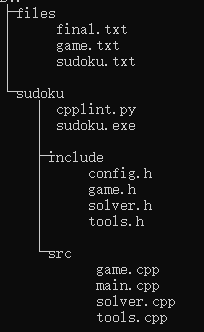
\includegraphics[scale=0.9]{images/tree.png}
    \caption{文件结构}
    \label{fig:tree}
\end{figure}
\par
其中,files为默认的txt文件输出路径;sudoku文件夹下存放着源文件与可执行文件。其中:
\begin{enumerate}
\item files为默认的txt文件输出路径
\item sudoku文件夹下存放着可执行文件,为程序的主体
\item cpplint文件是用于静态代码分析
\item include文件夹下包含着编译所需要的头文件,其中:config.h为各种宏定义等的声明;game.h为生成游戏与终局的函数声明;solver.h为求解游戏的相关函数声明;tools.h为其他函数可能用到的一些辅助函数声明。
\item src文件夹下,game、solver与tools三个文件为头文件声明函数的具体定义,包含了生成游戏、求解游戏、输出到文件等功能的具体逻辑。main.cpp中则主要是运行参数的接收与处理,从而实现不同的功能。

\end{enumerate}
\section{编程规范}
代码使用CppLint检测并消除代码中的不规范。

使用CppLint时检测出代码一系列不规范。以game.cpp为例(为使结果清楚简洁已将同一类型不规范消除至一个):
\begin{figure}[!ht]
  \centering
  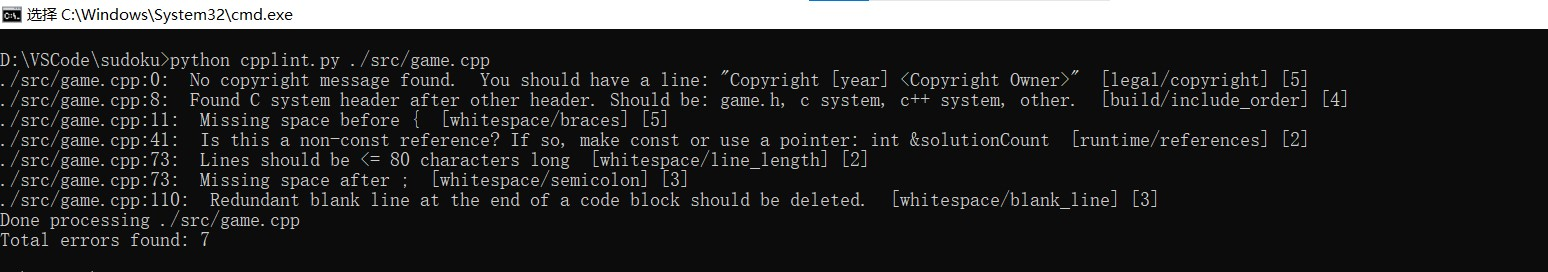
\includegraphics[scale=0.45]{images/ncpplint.jpg}
  \caption{编程不规范}
  \label{fig:ncpplint}
\end{figure}

包括:

\begin{enumerate}
	\item 无版权信息
	\item 缺少空格
	\item 代码行过长
	\item include头文件顺序错误
	\item 不允许函数参数为non-const 的reference
	\item 代码块末尾的多余空行未删除
\end{enumerate}

规范编程后实验结果如下:

\begin{figure}[!ht]
  \centering
  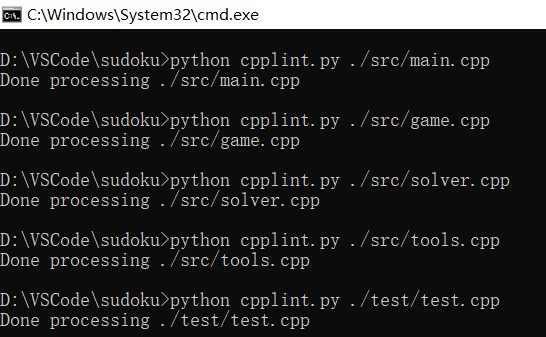
\includegraphics[scale=0.9]{images/cpplint.jpg}
  \caption{编程规范}
  \label{fig:cpplint}
\end{figure}

\section{质量分析}
\section{单元测试}
代码使用GoogleTest完成单元测试。GoogleTest是 Google 开源的一个跨平台C++ 单元测试框架。

代码分别就生成游戏的正确性、挖空范围、游戏难度、唯一解展开测试。
\begin{enumerate}
  \item 正确性。分别生成不同数量的唯一游戏,求解后测试解的正确性。
  \item 挖空范围。分别生成不同挖空数量的游戏,生成后测试挖空数量是否在设置的范围内。
  \item 游戏难度。分为生成不同难度的游戏,求解后测试游戏难度是否与初始设置一致。
  \item 唯一解。分别生成不同数量的唯一解游戏,求解后测试解的数量是否唯一。
\end{enumerate}

实验结果如下:

\begin{figure}[!ht]
  \centering
  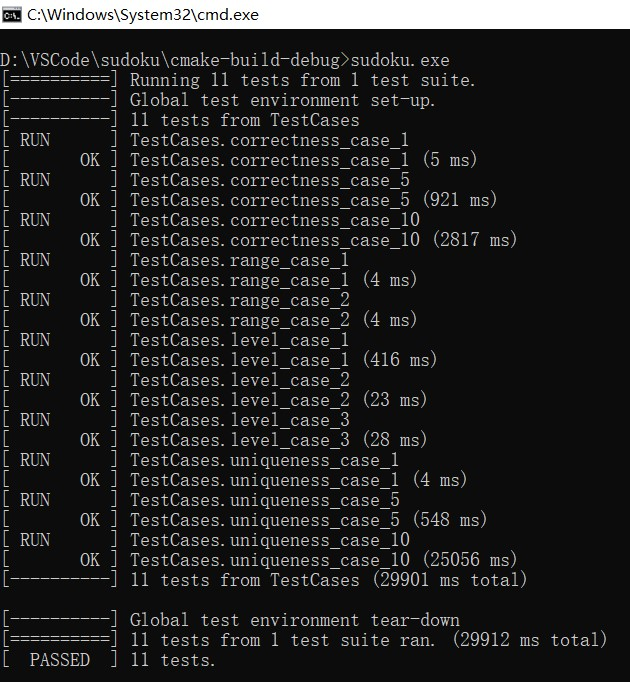
\includegraphics[scale=0.9]{images/test.jpg}
  \caption{单元测试}
  \label{fig:test}
\end{figure}


\section{覆盖统计}
\end{document}